\section{Approach}
\label{sec:approach}

The target of STSENet is to recover the missing contents in a corrupted video.
%
Our intuition is that there exists complementary information in neighboring frames, which can benefit the inpainting process of each individual frame.
Therefore, in each inference batch, to generate a complete frame \(Y_t\) at time $t$, total $5$ frames $\boldsymbol{X}$, indexed by $\msset{X}$, are fed to STSENet, as well as corresponding masks $\boldsymbol{M}$ that indicate the missing regions.
%Our method infers each target frame $Y_t$ individually but with hints from its neighboring source frames.
%
As shown in Fig.~\ref{fig:stiNet}, our STSENet mainly consists of three parts: (a) an edge inpainting network that recovers structural details of the input frames, (b) a flow inpainting network that completes the dense motions in the missing regions between neighbor frames and the target frame, and (c) a spatio-temporal inpainting network that generates plausible contents that looks spatially and temporally consistent.
The detailed implementation of each part will be explained in the following sections.

 



\subsection{Edge Inpainting Network}
\label{sec:edgenet}

Video inpainting suffers from the lack of structural details.
To inpaint the missing regions with fine details, we first predict their corresponding reasonable structural clues, which are beneficial to the following frame inpainting process.
%The edge completion module aims to generate the completed edge maps $\boldsymbol{E}$ for input frames $\boldsymbol{X}$. 
%

Given the input frames $\boldsymbol{X}$, we first extract their edge maps $\boldsymbol{E}^{i}$, of which there are no edges in the masked regions, using Canny edge detector. 
%Given the incompleted grayscale images $\boldsymbol{X}^{g}$ of input frame, a canny edge detector is first used to generate initial edge maps . 
Then, the edge inpainting network (ENet) completes the missing edges in $\boldsymbol{E}^{i}$.
The input of our ENet consists of the grayscale frames $\boldsymbol{X}^{g}$, initial edge maps $\boldsymbol{E}^{i}$, and their corresponding masks $\boldsymbol{M}$.
%
The detailed architecture of ENet is shown in Fig.~\ref{fig:stiNet}, which consists of a generator $G^E$ and a discriminator $D^E$.
$G^E$ contains a 2-layer 3D encoder, eight 2D residual blocks, and a 2-layer 3D decoder. 
The 3D encoder and decoder are designed to learn the spatial-temporal correlation, while the 2D residual blocks are used to enrich the spatial features in a larger receptive field. The discriminator $D^E$ follows the $70\times 70$ PatchGAN architecture \cite{Isola_2017_CVPR}. 
Finally, the inpainted edge maps are obtained by:
\begin{equation}
\label{eq:edgenet}
\boldsymbol{E}=G^E(\boldsymbol{E}^{i},\boldsymbol{X}^{g},\boldsymbol{M}),
\end{equation}

The ENet is trained by playing a minimax game to optimize the generator $G^E$ and the discriminator $D^E$ as
\begin{equation}
\label{eq:loss_e}
\min\limits_{G^E} \max \limits_{D^E} \big(\mathcal{L}^E_{adv}+\lambda_1 * \mathcal{L}^E_{fm}\big),
\end{equation}
where $\mathcal{L}^E_{adv}$ and $\mathcal{L}^E_{fm}$ are respectively the adversarial loss and feature matching loss. 
$\lambda_1$ is a hyper-parameter to balance the two terms.
%
Following the adversarial learning manner, $\mathcal{L}^E_{adv}$ can facilitate ENet to produce plausible edge maps, which is defined by
\begin{equation} \label{eq:edge_adver}
\mathcal{L}^E_{adv}  =\mathbb{E}\big[logD^E(\boldsymbol{E}^{gt},\boldsymbol{X}^{g})\big] +\mathbb{E} \big[log\big(1-D^E ( \boldsymbol{E},\boldsymbol{X}^{g})\big)\big],
\end{equation}
where $E^{gt}$ represents the ground truth edge maps. $\mathcal{L}^E_{fm}$ evaluates the feature-level similarity between ground truth edge maps and predicted edge maps, which helps to create structurally rational edge maps. 
\mdf{Feature matching loss has been widely used in recent GANs \cite{}... }
The feature matching loss is defined by:
\begin{equation}
\label{eq:edge_fm}
\mathcal{L}^E_{fm}=\sum_{k=1}^L{\frac{1}{N_k}\left\| D^E_k(\boldsymbol{E}^{gt},\boldsymbol{X}^{g})- D^E_k(\boldsymbol{E},\boldsymbol{X}^{g})\right\|_1},
\end{equation}
where $D^E_k$ is the output of the $k$-th layer in $D^E$, while $N_k$ is the element number of $D^E_k$. 
Note that the discriminator $D^E$ is not optimized by the feature matching loss term. It plays as a feature extractor to optimize the generator $G^E$ for producing plausible edge maps $\boldsymbol{E}$.




\subsection{Flow Inpainting Network}

It is vitally important to maintain temporal consistency in video inpainting.
To this end, we design a flow inpainting network (FNet) to predict the motion tendency among frames.
%
Similar to ENet, an initial flow maps \(\boldsymbol{O}^i\) for each group of neighboring frames $\boldsymbol{X}$ are first generated using an flow extraction network, such as FlowNet2.0~\cite{Flownet_2017_CVPR}.
Notably, \(\boldsymbol{O}^i\) consists of four flow maps \((O^i_{t\Rightarrow t-7}, O^i_{t\Rightarrow t-3}, O^i_{t\Rightarrow t+3}, O^i_{t\Rightarrow t+7})\) for the input 5 frames.
Then, the proposed FNet $G^F$ is used to complete \(\boldsymbol{O}^i\) by:
\begin{equation}
\label{eq:flownet}
\boldsymbol{O}=G^F(\boldsymbol{O}^{i},\boldsymbol{M}),
\end{equation}
where $\boldsymbol{O}$ denotes the predicted optical flows.
%
The detailed architecture of FNet is shown in Fig.~\ref{fig:stiNet}.

To train the flow inpainting network FNet, the loss function is given by:
\begin{equation}
\label{eq:flow_all}
\mathcal{L}_{flow}=\mathcal{L}^F_{rec}+ \mathcal{L}^F_{har},
\end{equation}
where $\mathcal{L}^F_{rec}$ and $\mathcal{L}^F_{har}$ are respectively $l_1$-reconstruction loss and hard mining loss, following the definition in \cite{Xu_2019_CVPR}. 
Specifically, $\mathcal{L}^F_{har}$ encourages the network to focus on those hard samples in order to avoid blurry texture.

%
%The $l_1$-reconstruction loss is defined as:
%\begin{equation}
%\label{eq:flow_l1}
%\mathcal{L}^F_{rec}=\frac{1}{\left\|\boldsymbol{M} \right\|_1}\left\|(\boldsymbol{O}-\boldsymbol{O}^{gt})\odot \boldsymbol{M}\right\|_1,
%\end{equation}
%where $\boldsymbol{O}^{gt}$ is the ground truth. The symbol $\odot$ denotes the pixel-wise multiplication. Specifically, $\mathcal{L}^F_{rec}$ measures the difference between $\boldsymbol{O}^{gt}$ and $\boldsymbol{O}$.
%The hard mining loss is defined as:
%\begin{equation}
%\label{eq:flow_hard}
%\mathcal{L}^F_{har}=\frac{1}{\left\|\boldsymbol{M}_H \right\|_1}\left\|(\boldsymbol{O}-\boldsymbol{O}^{gt})\odot \boldsymbol{M}_H\right\|_1,
%\end{equation}
%where $\boldsymbol{M}_H$ is the binary mask of hard example regions.
%The hard mining loss encourages the network to focus on those hard samples, which can avoid blurred texture. 

\subsection{Flow-Edge Consistency Loss}


Instead of separately training the two subnetworks ENet and FNet, we train the two networks jointly, because the temporal correlation and structural details can boost each other.
%, thereby rendering them to be mutually improved.
%Thus we will obtain detail-aware optical flow and temporal consistent edge maps.
To achieve this goal, a flow-edge consistency loss is defined as:
%
\begin{equation}
\label{eq:flow_edge}
\mathcal{L}_{fec}=\sum_{k}\frac{1}{\left\|M_{t} \right\|_1}\left\|(E_{t}-\phi(O_{t\Rightarrow t-k},E_{t-k}))\odot M_{t}\right\|_1,
\end{equation}
where $\phi(O_{t\Rightarrow t-k},E_{t-k})$ is the warping operation which warps the edge map $E_{t-k}$ to the target frame according to the generated optical flow $O_{t\Rightarrow t-k}$.
$k$ denotes the index of neighboring frames ($k\in \left\{-7,-3,+3,+7 \right\}$). 
%Specifically, $\mathcal{L}_{fec}$ warps the edge maps from neighboring frames to the target frame to penalize the reconstruction loss.
In terms of ENet, $\mathcal{L}_{fec}$ encourages the predicted edge maps to be temporally smoothing, which should conform to the motion tendency in the flow maps $\boldsymbol{O}$. 
In terms of FNet, $\mathcal{L}_{fec}$ constrains the model to focus on the edges in $\boldsymbol{E}$ by emphasizing edge motion in Eq.~\ref{eq:flow_edge}. 
Consequently, besides of the loss terms $\mathcal{L}_{edge}$ and $\mathcal{L}_{flow}$ for ENet and FNet respectively, $\mathcal{L}_{fec}$ further enhances them to obtain temporally consistent edges and edge-clear flows.
Thus, the total loss function for joint training of ENet and FNet is:
\begin{equation}
\label{eq:flow}
\mathcal{L}_{joint}=\mathcal{L}_{edge}+\mathcal{L}_{flow}+ \mathcal{L}_{fec}.
\end{equation}






\subsection{Spatio-Temporal Inpainting Network}

Combining the inpainted edge maps $\boldsymbol{E}$ and flow maps $\boldsymbol{O}$, a spatio-temporal inpainting network \mdf{(STINet)} is designed to obtain the final target frame $Y_t$.
\cxj{I modified to STINet to make it consistent with ENet and FNet. If it is ok, pls modify Fig 2 (STI Module) accordingly.}
%under the guidance of the edges and motion tendency, which is helpful to the completion process of the target frame...
Notably, the inpainted edges and flows provide structural details and temporal correlation, respectively.
To generate plausible video content, STINet adopts a coarse-to-fine architecture and consists of a coarse network and a refinement network, as shown in Fig.~\ref{fig:stiNet}.

%
The input of STINet is the concatenation of $\boldsymbol{X}$, $\boldsymbol{E}$, and $\boldsymbol{M}$.
First, the coarse network consists of a set of 3D convolutions to capture the temporal information, which targets to generate an initial rough completed frame with textures. 
The 3D coarse network is able to incorporate information from neighboring frames by convolution of the time dimension.
Second, the refinement network is implemented with 2D convolution layers to enhance structural details and refine the initial completed frame to produce a visually realistic frame with fine textures.

\begin{figure}[t]
	\centering
	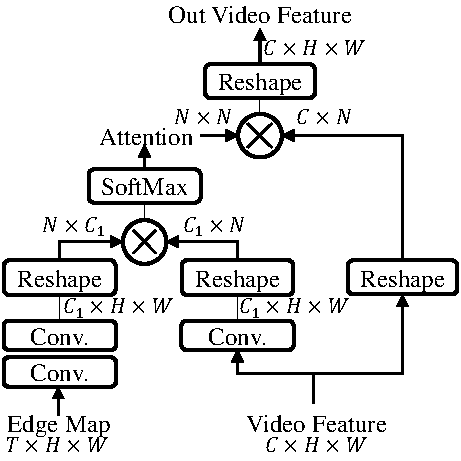
\includegraphics[width=0.65\columnwidth]{SEM} % Reduce the figure size so that it is slightly narrower than the column. Don't use precise values for figure width.This setup will avoid overfull boxes. 
	\caption{The architecture of SEM.}
	\label{SEM}
\end{figure}

To fully exploit the structural information in $\boldsymbol{E}$, a structure enhancement mechanism (SEM) is designed for STINet.
\cxj{Need one sentence to introduce the main concept of SEM here.}
As shown in Fig.~\ref{SEM}, two separate convolution blocks are first applied to $\boldsymbol{E}$.
Then, the input feature map and extracted structural information are interacted via matrix multiplication. 
Next, a SoftMax operation is used to obtain a normalized attention map.
Besides the short-range edge information in $\boldsymbol{E}$, the normalized attention map contains extra long-range correlation between structure and high-level features of video content.
Finally, the normalized attention map is applied to the original video features, and the structure information is thus encoded in the intermediate features of STI.
After introducing structure information, the inpainted video content by STI becomes more structure-preserved and semantically realistic.

To smooth temporal flickers and aggregate complementary neighboring clues, the motion tendency information in $\boldsymbol{O}$ is utilized by warping the neighboring frames into the target frame and employing a frame reconstruction constraint.
Specifically, a flow warping loss is proposed:
\begin{equation}
\label{eq:inp_flow}
\mathcal{L}^I_{flo}=\sum_{\widehat{t}\in\mathcal{T}}\left\| Y_t-\phi(O_{t\Rightarrow \widehat{t}},Y_{\widehat{t}}) \right\|_1,
\end{equation}
where $\mathcal{T}=\{t-7,t-3\}$. $\phi(O_{t\Rightarrow \widehat{t}},Y_{\widehat{t}})$ warps $Y_{\widehat{t}}$ to $Y_{t}$ using flow $O_{t\Rightarrow \widehat{t}}$.
Therefore, $\mathcal{L}^I_{flo}$ expects that all the neighboring frames can be well warped to the target frame with small reconstruction loss, rendering the inpainted frames to be temporal consistent.

%\(O_{t\Rightarrow t-3}\) is used to warp the inpainted $Y_{t-3}$ to aid the current $Y_{t}$, which provides a high temporal coherence.


%, which will generate a temporal smooth fine-detailed $Y_{t}$.
Finally, the loss function for STI is:
\begin{equation}
\label{eq:inpain_all}
\mathcal{L}_{inp}=\mathcal{L}^{I}_{rec}+\lambda_2 * \mathcal{L}^I_{adv}+ \mathcal{L}^I_{flo},
\end{equation}
where $\mathcal{L}^{I}_{rec}$, $\mathcal{L}^I_{adv}$, and $\mathcal{L}^I_{flo}$ are respectively reconstruction loss, adversarial loss and flow warping loss.


Inspired by \cite{nazeri2019edgeconnect}, $\mathcal{L}^{I}_{rec}$ consists of three terms by:
\begin{equation}
\mathcal{L}^{I}_{rec}=\mathcal{L}^{I}_{l1}+\lambda_3 *\mathcal{L}^{I}_{per}+\lambda_4 *\mathcal{L}^{I}_{sty},
\end{equation}
%\begin{equation}
%\begin{aligned}
%\mathcal{L}^{I}_{rec}=&\frac{1}{\left\|\boldsymbol{M} \right\|_1}\left\|(\boldsymbol{Y}^i-\widetilde{\boldsymbol{Y}})\odot \boldsymbol{M}\right\|_1 +\frac{1}{\left\|M_t \right\|_1}\left\|(Y_t-\widetilde{Y}_t)\odot M_t\right\|_1\\
%&+\mathbb{E}[\sum_{j}\frac{1}{N_j}\left\|\boldsymbol{\psi}_j(\widetilde{Y}_t)-\boldsymbol{\psi}_j(Y_t)\right\|_1]\\
%&+\mathbb{E}_j[\left\|G^{\boldsymbol{\psi}_j}(\widetilde{Y}_t)-G^{\boldsymbol{\psi}_j}(Y_t)\right\|_1],
%\end{aligned}
%\end{equation}
where the first term is pixel $l_1$ loss to evaluate generation quality. Different from \cite{nazeri2019edgeconnect}, we penalize both the coarse and fine predictions, which is defined by:
\begin{equation}
\begin{aligned}
\mathcal{L}^{I}_{rec}&=\frac{1}{\left\|\boldsymbol{M} \right\|_1}\left\|(\boldsymbol{Y}^i-\widetilde{\boldsymbol{Y}})\odot \boldsymbol{M}\right\|_1\\ &+\lambda_5*\frac{1}{\left\|M_t \right\|_1}\left\|(Y_t-\widetilde{Y}_t)\odot M_t\right\|_1.
\end{aligned}
\end{equation}
%

The second term is the perceptual loss \cite{gatys2015neural}, which compares the semantic contents between the generated frame and ground truth. The third term is the style loss, designed to prevent "checkerboard" artifacts \cite{Sajjadi_2017_ICCV} caused by transpose convolution.




%$\boldsymbol{\psi}_j$ denotes the activation maps of $j_{th}$ layer in a network. $N_j$ is the number of elements in layer $\boldsymbol{\psi}_j$. We use layers $relu_{1\_1}$, $relu_{2\_1}$, $relu_{3\_1}$, $relu_{4\_1}$ and $relu_{5\_1}$ of the VGG-19 network pre-trained on the ImageNet dataset for this loss.
%The third term is the style loss, designed to prevent "checkerboard" artifacts \cite{Sajjadi_2017_ICCV} caused by transpose convolution. $G^{\boldsymbol{\psi}_j}$ is the Gram matrix calculated by auto-correlation of $\boldsymbol{\psi}_j$. The layers are the same as that of perceptual loss.


$\mathcal{L}^I_{adv}$ is defined as:
\begin{equation}
\label{eq:inp_adver}
\mathcal{L}^I_{adv}=\min\limits_{G^I} \max \limits_{D^I}\mathbb{E}[logD^I(\widetilde{Y}_t)]+\mathbb{E}log[1-D^I(Y_{t})],
\end{equation}
where $G^I$ is the STI and $D^I$ possesses the same architecture as that of $D^E$, except the input dimension.